\begin{figure}[h]
	\begin{center}
    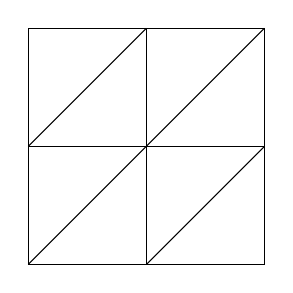
\begin{tikzpicture}[scale=0.5]
\tikzstyle{every node}=[font=\tiny]
      \draw (0,0) -- (6,0) -- (6,6) -- (0,6) -- cycle;
      \draw (0,0) -- (6,6);
      \draw (0,3) -- (6,3);
      \draw (3,0) -- (3,6);
      \draw (0,3) -- (3,6);
      \draw (3,0) -- (6,3);
    \end{tikzpicture}
	\end{center}
  \caption{Initial Mesh with $h=0.5$.}
	\label{fig:Mesh}
\end{figure}
